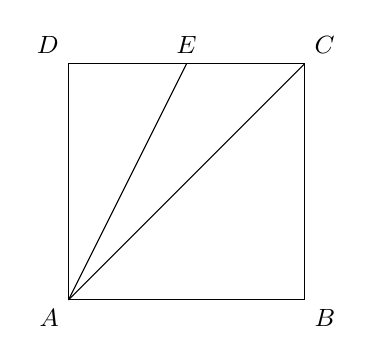
\begin{tikzpicture}[scale=.75, every node/.style={font=\small}]
  \coordinate (A) at (0,0); \coordinate (B) at (4,0);
  \coordinate (C) at (4,4); \coordinate (D) at (0,4);
  \coordinate (E) at (2,4);
  \draw (A)--(B)--(C)--(D)--cycle;
  \draw (A)--(C); \draw (A)--(E);
  \node[below left] at (A) {$A$};
  \node[below right] at (B) {$B$};
  \node[above right] at (C) {$C$};
  \node[above left] at (D) {$D$};
  \node[above] at (E) {$E$};
\end{tikzpicture}
